%! Author = k
%! Date = 2024/11/2

% Preamble
\documentclass[11pt]{article}

% Packages
\usepackage{amsmath}
\usepackage{tikz}
\usepackage{karnaugh-map}
\usetikzlibrary{karnaugh}

% Document
\begin{document}


    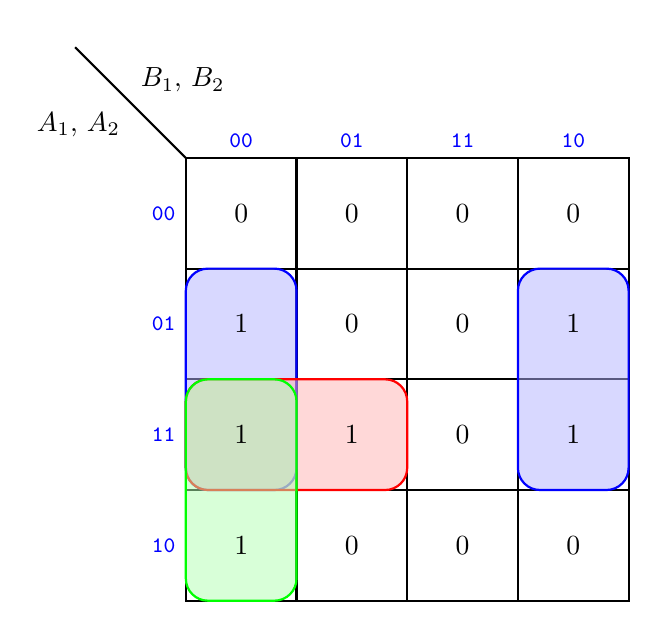
\begin{tikzpicture} [
        karnaugh,
        karnaugh cell size = 4em,
        American style,
        thick,
        grp/.style n args={3}{
        #1,fill=#1!30,
        minimum width=#2\kmunitlength,
        minimum height=#3\kmunitlength,
        rounded corners=0.2\kmunitlength,
        fill opacity=0.5,
        rectangle,draw
        }
    ]

        % 一个格子是4em

    \karnaughmaptab{4}{}{{$A_1$}{$A_2$}{$B_1$}{$B_2$}} {
        0000 1001 1101 1000
    } {
        \node[grp = {blue}{1}{2}](n001) at (2em,8em) {};
        \node[grp = {blue}{1}{2}](n001) at (14em,8em) {};
        \node[grp = {red}{2}{1}](n001) at (4em,6em) {};
        \node[grp = {green}{1}{2}](n001) at (2em,4em) {};
    }

    \end{tikzpicture}




\end{document}